\documentclass[tikz,border=3pt]{standalone}
\usepackage[T1]{fontenc}
\usepackage{mathptmx}
\usepackage{tikz,pgfplots}
\usetikzlibrary{arrows.meta,positioning,calc,fit,backgrounds,shapes.geometric}
\pgfplotsset{compat=1.18}
\definecolor{forest}{HTML}{346E57}
\definecolor{sage}{HTML}{E8EFEA}
\definecolor{clay}{HTML}{AC653F}
\definecolor{sand}{HTML}{F4EAE2}
\definecolor{ink}{HTML}{252525}
\definecolor{light}{HTML}{F5F5F3}
\definecolor{gridgray}{HTML}{D8DAD6}
\tikzset{box/.style={draw=ink!70,line width=.5pt,rectangle,rounded corners=1pt,fill=white,align=center,font=\fontsize{11}{12}\selectfont,inner sep=6pt}, flow/.style={-{Latex[length=2.4mm]},line width=.7pt,draw=ink!80}, data/.style={flow,densely dashed,draw=forest}, label/.style={font=\fontsize{10}{11}\selectfont,fill=white,inner sep=2pt,align=center}}
\hyphenpenalty=10000\exhyphenpenalty=10000\begin{document}
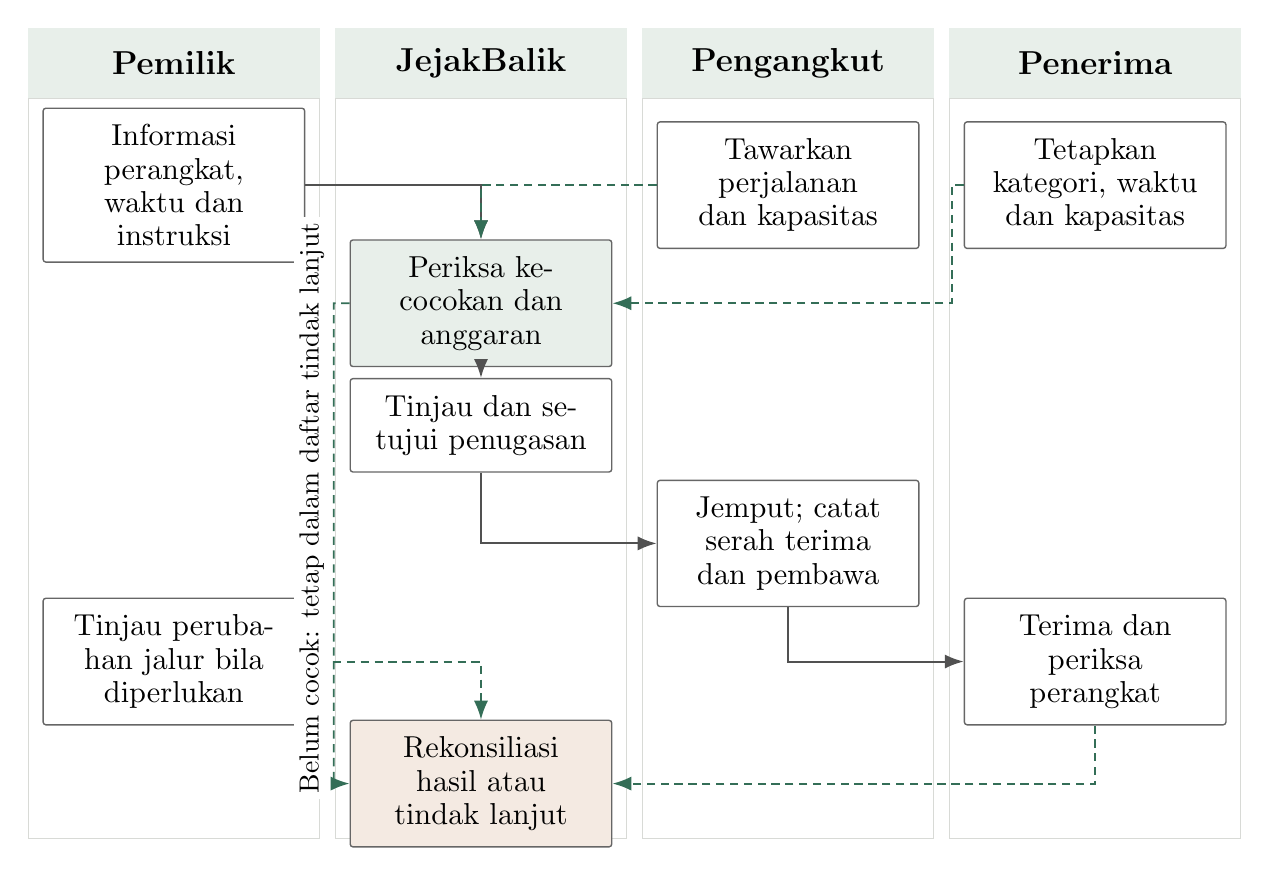
\begin{tikzpicture}[x=1cm,y=1cm]
\foreach \x/\title in {0/{Pemilik},3.9/{JejakBalik},7.8/{Pengangkut},11.7/{Penerima}}{
\fill[sage] (\x-1.85,0) rectangle(\x+1.85,.9);\node[font=\fontsize{12}{14}\selectfont\bfseries]at(\x,.45){\title};
\draw[gridgray] (\x-1.85,-9.4)rectangle(\x+1.85,0);}
\node[box,text width=2.9cm](input)at(0,-1.1){Informasi perangkat, waktu dan instruksi};
\node[box,text width=2.9cm](offers)at(7.8,-1.1){Tawarkan perjalanan dan kapasitas};
\node[box,text width=2.9cm](accept)at(11.7,-1.1){Tetapkan kategori, waktu dan kapasitas};
\node[box,text width=2.9cm,fill=sage](match)at(3.9,-2.6){Periksa kecocokan dan anggaran};
\node[box,text width=2.9cm](review)at(3.9,-4.15){Tinjau dan setujui penugasan};
\node[box,text width=2.9cm](pickup)at(7.8,-5.65){Jemput; catat serah terima dan pembawa};
\node[box,text width=2.9cm](receive)at(11.7,-7.15){Terima dan periksa perangkat};
\node[box,text width=2.9cm](decision)at(0,-7.15){Tinjau perubahan jalur bila diperlukan};
\node[box,text width=2.9cm,fill=sand](close)at(3.9,-8.7){Rekonsiliasi hasil atau tindak lanjut};
\draw[flow](input.east)-|(match.north);\draw[data](offers.west)-|(match.north);\draw[data](accept.west)--++(-.15,0)|-(match.east);
\draw[flow](match)--(review);\draw[flow](review.south)|-(pickup.west);\draw[flow](pickup.south)|-(receive.west);
\draw[data](receive.south)|-(close.east);\draw[data](decision.east)--(3.9,-7.15)--(close.north);
\draw[data](match.west)--++(-.2,0)--++(0,-6.1)--(close.west);
\node[label,rotate=90]at(1.75,-5.2){Belum cocok: tetap dalam daftar tindak lanjut};
\end{tikzpicture}
\end{document}
